\section{Hardware components}
In the very beginning of the project, the team looked into the possibility of getting live data directly from devices. This required some technical equipment for collecting and transmitting the usage of a device. The idea was that the app should get live data directly form all of the devices in a house, and if possible control the devices. With such a device it is possible to modify Wattitude to receive data from the hardware device.

\subsection{Home data aggregator}
To ensure full operability 24 hours a day, a base station is needed in the user's home. This server will serve as an aggregating agent for data from measuring devices spread around the residence. Given an ideal architecture implementation, this unit would also be responsible for controlling devices. The team envisions this unit as a REST service mostly running synchronizations towards the Wattitude cloud server. The software for such a server could be based on the current server software. The ideal hardware for a this base station would be a Raspberry pi. These computers are very cheap, and provides all that is needed in a small board that can be hidden away. Modifications might be needed to interface with the measuring devices. 

\begin{figure}[H]
\centering
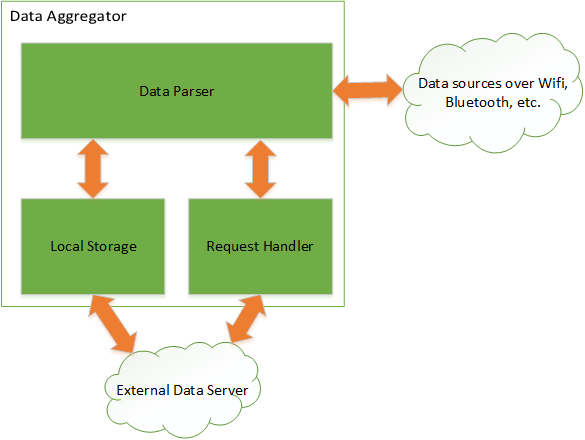
\includegraphics[height=0.4\textheight]{ch/further/fig/home.png}
\caption{Detailed architecture for the home data aggregator.}
\label{fig:aggregator}
\end{figure}

\subsection{Measuring device}
To make real time monitoring possible, every device that the user wants to monitor must be connected to a wireless monitoring device. The team tried to find a conclusive answer to what the best solution would be, but every option we found had enough flaws to dethrone it from a recommendation. The following are a couple of the most viable options.

\paragraph{HomeMatic plug}
This is the device that the Cossmic team at Sintef has been experimenting with. The first drawbacks are that it must be ordered from Germany, and that it has a unit price of almost 500NOK. Covering most home devices with such a measuring device would be extremely costly. It is part of the HomeMatic proprietary hardware line, and is meant to interface with a HomeMatic central control unit, much like the base station we have described above. As hardware devices were not a part of the project scope, the team did not do any research on how to interface with this unit. The only knowledge we have is that the Sintef team working on Cossmic has been working on it.

\paragraph{DIY Arduino}
A much cheaper, but perhaps limited solution is one from Open Energy Monitor~\cite{oemmodule}. These units do not allow for control of devices, only measurement of consumption. They are much cheaper than the HomeMatic unit, but must be assembled manually and can not control devices. A modification of these units with a relay may enable the desired functionality.